% Section 3 of the CIRP CMS paper: architecture and method. Rewritten 3 Nov 2026 from the draft of
% 1 Nov, in the terms of the abstract and the introduction (product, process and resource AAS;
% parameter, flow and structural changes), with the related work placed where each design choice is
% made.
%
% "DD n" in the comments points to docs/design-decisions.md. The paper cites at most 17 sources, those
% of references.bib beside this file; PackML, 4diac FORTE and IDTA 02017 are named, not cited. Budget:
% about two pages with Figs. 1 to 3; paragraphs marked "% cut first" are the first to go.
%
% Figures: figures/*.pdf beside this file, the pages of docs/figures/cirp-figures.drawio (export:
% docs/figures/export_pdf.py). Fig. 3 is the page product-to-process since 3 Nov; the page
% planned-skill is told in the text instead (swap back: figures/planned-skill.pdf).
%
% Terms: module, component; primitive skill, composite skill; requirement, flow; described, built;
% verify, reconfigure, record.

\section{Architecture and method}
\label{sec:method}

\subsection{The AAS as the desired state}
\label{sec:concept}

% DD 1.1, 1.4; ppr-model.md, section 1
The approach follows the product--process--resource paradigm, with an AAS for each
(Fig.~\ref{fig:concept}). A product's AAS states the processes the product requires, the capability
each requires and its parameters, such as a fill volume. The process AAS binds the product's procedure
to the line: each step to a module and one of its skills, with the parameters' values. A module's
resource AAS describes its skills, their interfaces, the capabilities they offer, and which of them
the module's IEC~61499 program carries out~\cite{iec61499}. The resource AAS is that program's desired
state: a change of the module's behaviour is a change of its AAS, which a reconciler then applies to
the running program, verifies by reading the program back, and records.

% DD 1.1, 1.2. Cut first: from "Behaviour has three levels" to the end (section 3.3 gives the hierarchy).
The AAS is the source because every module comes with it and every client already reads
it~\cite{jensen2026service}, whereas code generators start from engineering models of the vendor or
the plant~\cite{dorofeev2021orchestrator,terzimehic2021service}, which an integrator seldom has. The
program is changed only over the IEC~61499 management protocol and operated only over OPC~UA, so
operating never changes the module; changes are made between products. Behaviour has three levels,
each composing only the one below, as device primitives, skills and tasks do in~\cite{schou2018skill}:
components (an axis, a pump, a scale) offer primitive skills, a module composes them into composite
skills, and the line, outside this paper, orchestrates the modules'
skills~\cite{jensen2026service,schwoerer2026fond}.

\begin{figure*}[t]
  \centering
  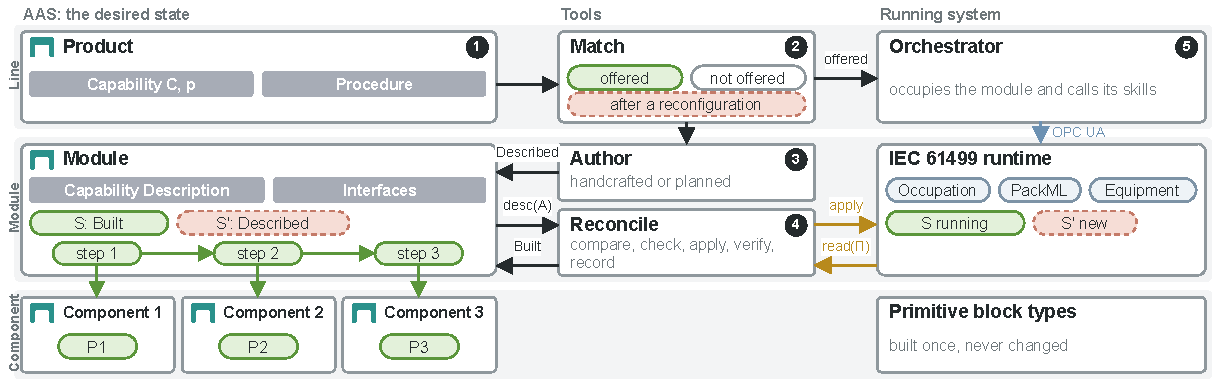
\includegraphics[width=\textwidth]{figures/pipeline.pdf}
  \caption{The AAS as the desired state of the module's IEC~61499 program, over the three levels
    (rows). (1)~A product requires a capability, and (2)~matching answers offered, offered after a
    reconfiguration, or not offered. (3)~A new skill is written or planned and enters the module's AAS
    as Described. (4)~The reconciler compares the running program with the AAS, applies the change
    online over the management protocol, verifies it by reading the program back and records it as
    Built. (5)~The orchestrator calls the skill over OPC~UA. The baseline is a new boot file and a
    restart.}
  \label{fig:concept}
\end{figure*}

\subsection{Module architecture}
\label{sec:architecture}

The module's program follows fixed rules that make a composite skill data rather than code
(Fig.~\ref{fig:mapping}).

% DD 2.2, 2.8, 2.9
\emph{The shell} is the same in every module and does not change online: an occupation block, which
lets one client at a time command the module; a PackML state machine for the module; one block per
equipment item, which owns the item's IO and enforces only what every writer must respect (one
holder, break before make, all off on release or abort); and one initialisation chain. The control
components used in~\cite{dorofeev2021orchestrator} also combine an occupation with a PackML-based
execution state. In the Module Type Package, every service runs a full state machine of 16
states~\cite{huang2026plug}; here PackML runs once, for the module, and a skill has a smaller machine
of its own.

% DD 2.2, 2.4, 2.5, 2.7
\emph{A primitive skill} is a block type, built into the runtime once and never changed. It sends one
command to one equipment item until a sensor condition holds or a time has passed, within a timeout.
\emph{Every skill}, primitive or composite, has the same state machine (Idle, Running, Stopping,
Succeeded, Failed, Aborted) and OPC~UA methods (Start, Stop, Abort, Reset), which answer at once
whether a call is accepted. A skill is called, runs and ends, like a node of a behaviour tree; its
parameters are the arguments of Start, range-checked before anything moves.

% DD 2.4, module rules section 3 (rule set 2)
\emph{A composite skill} has no type of its own. It is a subapplication of instances only: a library
block for its state machine and methods, a latch per parameter that checks its range and holds its
default, and an instance of a primitive per step, named like the step and holding its constants. Steps
are chained by their success events and their failures merged; a parallel block adds a join, a
decision a comparison and a merge. The rules derive all wiring from the flow alone.

% DD 2.4. Cut first: the last sentence ("And each step stays an instance ...").
Instances, not a type per composite, because every IEC~61499 runtime creates instances and connections
online through the management commands~\cite{iec61499}, while a new type needs a build or a type
loader (4diac FORTE loads one only with its Lua loader). A generated type also grows to $2^n$ states for
$n$ parallel branches~\cite{dorofeev2021orchestrator}, whereas a join grows linearly, like the
rendezvous blocks of the applications generated in~\cite{terzimehic2021service}. And each step stays an
instance that can be read back and watched in the IDE, which a sequence interpreted in one generic
block, such as a behaviour-tree engine, would not be.

% DD 2.3, 2.9
\emph{A new composite touches nothing that runs.} Blocks reach the equipment, the occupation and the
module's release over the runtime's local publish/subscribe channels, not over connections, so a
composite created online needs one connection only, at the end of the initialisation chain.
Reconfiguration services keep the rest of an application running while a part of it
changes~\cite{rooker2007zero}; here zero downtime holds by construction.

% DD 2.10; DD 1.3 for the last sentence. Cut first: the last sentence (the rules as the contract).
\emph{What may change online} follows. Huang et al. grade online reconfiguration into connections and
parameters, instances, and types~\cite{huang2026plug}; our three classes run along the same lines. A
\emph{parameter} change (a default, a limit, a step's constant) is written online while the module is
neither executing nor occupied. A \emph{flow} change that adds a composite is made online in any state;
one that reorders or removes a composite deletes instances a running skill may hold, and needs a
restart. A \emph{structural} change (a new primitive, equipment item or IO) needs new block types and a
build. The rules, not our generator, are the contract, so a module written by hand in the same form is
read and changed alike.

\begin{figure}[t]
  \centering
  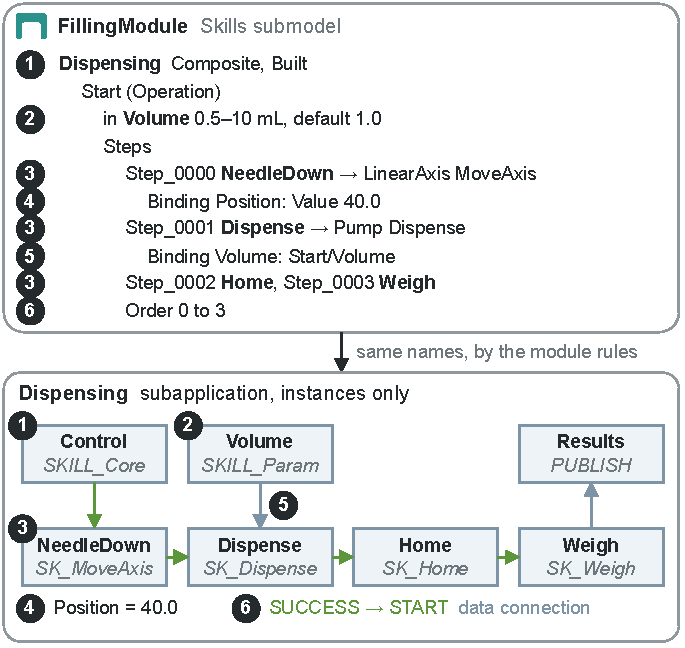
\includegraphics[width=\columnwidth]{figures/aas-to-blocks.pdf}
  \caption{A composite skill in the AAS and the blocks it becomes, joined by name. Dispensing is a
    subapplication of instances only: (1)~the skill gives its control block, (2)~a parameter a latch,
    (3)~a step an instance of its primitive's type, (4)~a bound value an input's value, (5)~a bound
    parameter a connection from the latch, and (6)~the order of the steps the chain of their events.}
  \label{fig:mapping}
\end{figure}

\subsection{Skills and products in the AAS}
\label{sec:aas}

% DD 3.2, 3.3; module rules section 5. Cut first: the last two sentences (one format, BPMN).
\emph{The skill hierarchy.} Skills are described in a Skills submodel, as in~\cite{blumhofer2025enhancing},
where the AAS describes each skill's interface and conditions but leaves its composition inside the
machine. Here the composition is described too: primitives are in their component's AAS, composites in
the module's, and a composite's steps refer to the components' primitives. A skill is a collection of commands, each an Operation whose
inputs are the parameters, with unit, limits, default and meaning, and whose outputs are the results;
each refers to the action of the module's Asset Interfaces Description (IDTA 02017) that calls it. A
composite's Start command holds its flow, written in the elements of a product's procedure: steps with
their order and skill, bindings of constants and parameters, parallel blocks, decisions and conditional
steps. One format serves products and skills. Both are drawn in BPMN, as skill sequences are
in~\cite{lindorfer2019user}, but kept block-structured, so that every flow maps to blocks.

% module rules section 5
\emph{Translation rules} join the AAS and the program by name (Fig.~\ref{fig:mapping}): a skill is the
subapplication of the same name, a step the instance, a parameter the latch. Three things are thus
inferred, not described: a composite's wiring, from its flow; a running program's skills, from reading
it back; and the capability a skill offers, from its steps.

% DD 3.4, 3.7; ppr-model.md, section 5
\emph{Capabilities derived from skills.} The offered capabilities in the module's Capability
Description~\cite{idta02020} are derived from its skills: a skill offers the capability its primitives
contribute to, with ranges from its parameters' meanings and limits, and a composite that repeats a
step offers what it reaches when run through the module's states (two doses of 0.5--10\,mL offer
1--20\,mL). A capability therefore cannot drift from its skill.

% ppr-model.md, sections 4 and 8
\emph{The product hierarchy} uses the same references (Fig.~\ref{fig:product}). A product's process
requires a capability with its parameters. Matched against the module's offered capabilities, it is
offered, not offered, or offered after a reconfiguration, by a skill that is \emph{Described} in the AAS
but not yet \emph{Built}. The process AAS then binds the product's step to the module and the skill.
Albus et al. also match a product's required capabilities against the resources'~\cite{albus2025automated},
but to assign skills that exist; here the third answer leads to a new skill.

\begin{figure}[t]
  \centering
  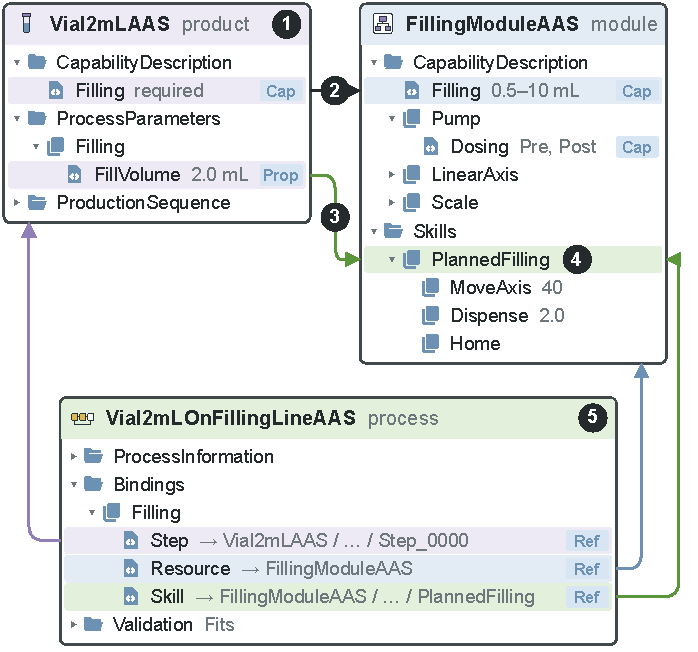
\includegraphics[width=\columnwidth]{figures/product-to-process.pdf}
  \caption{From a product's need to a new skill. (1)~The 2\,mL vial requires Filling with a FillVolume
    of 2.0\,mL; (2)~the module offers Filling for 0.5--10\,mL. (3)~From the requirement the module
    plans PlannedFilling from its components' capabilities, and (4)~builds it online. (5)~The process
    AAS binds the product's step to the module and the skill, and records that it fits.}
  \label{fig:product}
\end{figure}

\subsection{Two routes to a new skill, and the check}
\label{sec:authoring}

A new composite enters the AAS as a described skill, by one of two routes, and is checked before
anything is deployed.

% DD 4.7, G3 and G7. Cut first: the syringe example (section 4 tells it).
\emph{Handcrafted:} the skill editor, a web application on the AAS server, draws a composite as a flow
of the module's primitives. Filling a syringe from the bottom was written so: the needle goes deep,
then rises while the pump doses.

% DD 3.9, 4.8. Cut first: "Each property names the data point ...".
\emph{Planned from the product's recipe:} when the match answers not offered, the module plans a
composite from its Capability Description~\cite{idta02020}. Besides the offered capabilities, it holds a
capability set per component, each capability realized by a primitive, with pre- and postconditions and
invariants as the template's property constraints: for dosing, the needle must be at the fill position
or deeper before and while it runs, and the content grows by the volume dosed. Each property names the
data point it stands for, so the planner and the primitives' run-time conditions refer to the same
signals. The planner combines hierarchical task networks with goal regression~\cite{nau2021gtpyhop}:
stated compositions are tried first; otherwise each goal is reached by a component capability whose
postcondition achieves it, after that capability's own precondition, ending in the module's rest
state. The plan is lifted to a partial order, steps on different components with no state between
them becoming a parallel block unless an invariant forbids it; a volume above one dose becomes two
doses. Approaches that generate PDDL add planning submodels to the AAS~\cite{nabizada2026capability};
here nothing planning-specific is added, since inside one module the state is a handful of values and
the standard constraints already say what each capability needs and does.

% DD 4.7, 3.4; skill-planning.md, section 10 (T6, T7)
\emph{The check.} Every flow, written or planned, is run through the module's capability model. A
condition that does not hold is reported with the step at which it fails and a step that would make it
hold, such as a dose without the needle in the vial, or weighing while the axis moves. Lindorfer and
Froschauer refuse invalid sequences by rules that a tool expert writes~\cite{lindorfer2019user}; here
the rules are the capabilities' conditions, which the AAS holds already. The capability the flow offers
is then derived and matched against the product's requirement, and only a skill that fits is offered to
the product, before anything is deployed.

\subsection{Reconciling the running program}
\label{sec:reconcile}

% DD 4.1
Let $\Pi$ be the running program and $A$ the module's AAS. The reconciler reads $\Pi$ back over the
management protocol, which reports every instance, connection, type hash and value, and parses it by
the rules into skills, steps, constants and types, $\mathit{read}(\Pi)$; the AAS gives the same
structure, $\mathit{desc}(A)$. The module is verified when
\begin{equation}
  \mathit{read}(\Pi) = \mathit{desc}(A).
  \label{eq:verify}
\end{equation}
Otherwise the differences are sorted into the three classes, and a reconfiguration applies the least
disruptive change and proves it:
\begin{enumerate}
  \item \emph{Compare} and \emph{check}: the steps name primitives the module has, bound values lie
    within their limits, and the AAS passes the ontology's checks; a missing block type refuses the
    change before anything is sent.
  \item \emph{Guard} and \emph{apply}: what the class allows is applied online by management commands,
    values only while the module is neither executing nor occupied; the rest is refused as needing a
    restart or a build.
  \item \emph{Verify}: the program is read back, and Eq.~(\ref{eq:verify}) is evaluated again.
  \item \emph{Record}: the change is added to the boot file, so that it survives a restart, and the
    skill is marked Built in the AAS with its interface, which clients follow by reference.
\end{enumerate}

% DD 4.2, 4.4. Cut first: the last sentence (identical by construction).
Huang et al. compare the runtime with the MTP file before they send commands~\cite{huang2026plug};
here the program is also read back afterwards, so a command lost or refused shows as a difference. The
commands that create a composite come from the function the generator uses, so a program changed
online and one generated with the skill are identical by construction.
